% %%「論文」，「レター」，「レター（C分冊）」，「技術研究報告」などのテンプレート
% %% v3.4 [2023/09/12]
% %% 1. 「論文」
% \documentclass[paper]{ieicej}
% %\documentclass[invited]{ieicej}% 招待論文
% %\documentclass[survey]{ieicej}% サーベイ論文
% %\documentclass[comment]{ieicej}% 解説論文
% %\usepackage[dvipdfmx]{graphicx,xcolor}
% %%\usepackage[dvips]{graphicx}
% \usepackage[fleqn]{amsmath}
% %\usepackage{amsthm}
% \usepackage{newtxtext}% 英数字フォントの設定を変更しないでください
% \usepackage[varg]{newtxmath}% % 英数字フォントの設定を変更しないでください
% %\usepackage{amssymb}
% %\usepackage{bm}

% \setcounter{page}{1}

% \field{A}
% \jtitle{論文題目}
% \etitle{Title in English}
% \authorlist{%
%  \authorentry{林 奏汰}{Sota Hayashi}{Osaka}\MembershipNumber{}
%  %\authorentry{和文著者名}{英文著者名}{所属ラベル}\MembershipNumber{}
%  %\authorentry[メールアドレス]{和文著者名}{英文著者名}{所属ラベル}\MembershipNumber{}
%  %\authorentry{和文著者名}{英文著者名}{所属ラベル}[現在の所属ラベル]\MembershipNumber{}
% }
% \affiliate[Osaka]{UOsaka}{Uosaka}
% %\affiliate[所属ラベル]{和文所属}{英文所属}
% %\paffiliate[]{}
% %\paffiliate[現在の所属ラベル]{和文所属}
% \jalcdoi{???????????}% ← このままにしておいてください

% \begin{document}
% \begin{abstract}
%     dfhjかsdhふあsdhふはsdjkfはsdhjkfh
% %和文あらまし 500字以内
% \end{abstract}
% \begin{keyword}
% %和文キーワード 4〜5語
% \end{keyword}
% \begin{eabstract}
% %英文アブストラクト 100 words
% \end{eabstract}
% \begin{ekeyword}
% %英文キーワード
% \end{ekeyword}
% \maketitle

% \section{まえがき}


% \ack %% 謝辞

% %\bibliographystyle{sieicej}
% %\bibliography{myrefs}
% \begin{thebibliography}{99}% 文献数が10未満の時 {9}
% \bibitem{}
% \end{thebibliography}

% \appendix
% \section{}

% % 著者紹介・顔写真の掲載はC分冊の場合は任意です．
% \begin{biography}
% \profile{a}{林 奏汰}{現在，大阪大学大学院在学．}
% %\profile{会員種別}{名前}{紹介文}% 顔写真あり
% %\profile*{会員種別}{名前}{紹介文}% 顔写真なし
% \end{biography}

% \end{document}



% %% 2. 「レター」
% \documentclass[letter]{ieicej}
% %\usepackage[dvipdfmx]{graphicx,xcolor}
% %%\usepackage[dvips]{graphicx}
% \usepackage[fleqn]{amsmath}
% %\usepackage{amsthm}
% \usepackage{newtxtext}% 英数字フォントの設定を変更しないでください
% \usepackage[varg]{newtxmath}% % 英数字フォントの設定を変更しないでください
% %\usepackage{amssymb}
% %\usepackage{bm}

% \setcounter{page}{1}

% \typeofletter{研究速報}
% %\typeofletter{紙上討論}
% %\typeofletter{問題提起}
% %\typeofletter{ショートノート}
% \field{}
% \jtitle{}
% \etitle{}
% \authorlist{%
%  \authorentry{}{}{}{}\MembershipNumber{}
%  %\authorentry{和文著者名}{英文著者名}{会員種別}{所属ラベル}\MembershipNumber{}
%  %\authorentry{和文著者名}{英文著者名}{会員種別}{所属ラベル}[現在の所属ラベル]\MembershipNumber{}
% }
% \affiliate[]{}{}
% %\affiliate[所属ラベル]{和文所属}{英文所属}
% %\paffiliate[]{}
% %\paffiliate[現在の所属ラベル]{和文所属}
% \jalcdoi{???????????}% ← このままにしておいてください

% \begin{document}
% \maketitle
% \begin{abstract}
% %和文あらまし 120字以内
% \end{abstract}
% \begin{keyword}
% %和文キーワード 4〜5語
% \end{keyword}
% \begin{eabstract}
% %英文アブストラクト 50 words
% \end{eabstract}
% \begin{ekeyword}
% %英文キーワード
% \end{ekeyword}

% \section{まえがき}


% \ack %% 謝辞

% %\bibliographystyle{sieicej}
% %\bibliography{myrefs}
% \begin{thebibliography}{99}% 文献数が10未満の時 {9}
% \bibitem{}
% \end{thebibliography}

% \appendix
% \section{}

% \end{document}



% %% 3. 「レター（C分冊）」
% \documentclass[electronicsletter]{ieicej}
% %\usepackage[dvipdfmx]{graphicx,xcolor}
% %%\usepackage[dvips]{graphicx}
% \usepackage[fleqn]{amsmath}
% %\usepackage{amsthm}
% \usepackage{newtxtext}% 英数字フォントの設定を変更しないでください
% \usepackage[varg]{newtxmath}% % 英数字フォントの設定を変更しないでください
% %\usepackage{amssymb}
% %\usepackage{bm}

% \setcounter{page}{1}

% \field{}
% \jtitle{}
% \etitle{}
% \authorlist{%
%  \authorentry{}{}{}{}\MembershipNumber{}
%  %\authorentry{和文著者名}{英文著者名}{会員種別}{所属ラベル}\MembershipNumber{}
%  %\authorentry{和文著者名}{英文著者名}{会員種別}{所属ラベル}[現在の所属ラベル]\MembershipNumber{}
% }
% \affiliate[]{}{}
% %\affiliate[所属ラベル]{和文所属}{英文所属}
% %\paffiliate[]{}
% %\paffiliate[現在の所属ラベル]{和文所属}
% \jalcdoi{???????????}% ← このままにしておいてください

% \begin{document}
% \begin{abstract}
% %和文あらまし 120字以内
% \end{abstract}
% \begin{keyword}
% %和文キーワード 4〜5語
% \end{keyword}
% \begin{eabstract}
% %英文アブストラクト 50 words
% \end{eabstract}
% \begin{ekeyword}
% %英文キーワード
% \end{ekeyword}
% \maketitle

% \section{まえがき}


% \ack %% 謝辞

% %\bibliographystyle{sieicej}
% %\bibliography{myrefs}
% \begin{thebibliography}{99}% 文献数が 10 未満の時 {9}
% \bibitem{}
% \end{thebibliography}

% \appendix
% \section{}

% \end{document}



%% 4. 「技術研究報告」
\documentclass[technicalreport]{ieicej}
\usepackage[dvipdfmx]{graphicx,xcolor}
%%\usepackage[dvips]{graphicx}
\usepackage[fleqn]{amsmath}
% \usepackage{amsthm}
\usepackage{newtxtext}% 英数字フォントの設定を変更しないでください
\usepackage[varg]{newtxmath}% % 英数字フォントの設定を変更しないでください
%\usepackage{amssymb}
%\usepackage{bm}
\usepackage{stfloats}

\tecrepyear{2026}% X を適宜書き換えてください
\jtitle{反応時間の変動を指標とした暗黙的学習における個人差の検討}
\jsubtitle{}
\etitle{Individual Differences in Implicit Learning Measured by Reaction Time Variability}
\esubtitle{}
\authorlist{%
 \authorentry{林 奏汰}{Sota Hayashi}{Osaka}
 \authorentry{原 惇也}{Junya Hara}{Osaka}
 \authorentry{田中 雄一}{Yuichi Tanaka}{Osaka}
 \authorentry{東 広志}{Hiroshi Higashi}{Kansai}
% \authorentry[メールアドレス]{和文著者名}{英文著者名}{所属ラベル}
}
\affiliate[Osaka]{大阪大学大学院工学研究科 〒565-0871 大阪府吹田市山田丘2-1}{Graduate School of Engineering, The University of Osaka, 2-1 Yamadaoka, Suita, Osaka 565-0871, Japan}
\affiliate[Kansai]{関西大学 システム理工学部 〒564-0073 大阪府吹田市山手町3-3-35}{Faculty of Engineering Science, Kansai University, 3-3-35 Yamate-cho, Suita, Osaka 564-8680, Japan}
%\affiliate[所属ラベル]{和文勤務先\\ 連絡先住所}{英文勤務先\\ 英文連絡先住所}

% emailを赤林のを参考にして一行で書く
\MailAddress{$\dagger$s.hayashi@sip.comm.eng.osaka-u.ac.jp, j.hara@comm.eng.osaka-u.ac.jp, ytanaka@comm.eng.osaka-u.ac.jp $\dagger\dagger$hgshrs@kansai-u.ac.jp}

\begin{document}
\begin{jabstract}
% 集中状態と注意状態の定義がごっちゃになっていて，アブストとイントロ
人は，環境に潜む規則性を意識せずとも自然に習得する能力を有しており，これは暗黙的学習と呼ばれる．
暗黙的学習の進行過程には顕著な個人差が認められるが，その要因については十分に解明されていない．
本研究では，集中度（注意状態）の個人差が学習の進行に影響を及ぼすと仮定し，集中度を反映する指標である反応時間の変動と暗黙的学習の進行度の関係を検討した．
ヒトを対象とした行動実験（$N=54$）では，白・黒のドット群がそれぞれ異なる方向に運動するランダムドットキネマトグラム刺激を用いた．
実験参加者は，白か黒のどちらかを選択し，その色のドット群の運動方向を報告し，選択ドットと運動方向誤差に応じて報酬を得た．
ドット群の選択には暗黙的な報酬構造が設定されており，参加者はこの報酬構造を学習することでより多くの報酬を獲得することが可能であった．
分析の結果，反応時間の変動が大きい参加者群において，課題の進行にともない高報酬なドット群を選択する割合が有意に増加することが確認された．
反応時間の変動は集中状態と散漫状態の遷移を反映していると考えられることから，
本結果は注意状態の動的な変化が暗黙的学習の進行を規定する要因になり得ることを示唆している．
%和文あらまし
\end{jabstract}
\begin{jkeyword}
%和文キーワード
暗黙的学習，注意状態，反応時間，変動係数，報酬構造，ランダムドットキネマトグラム
\end{jkeyword}
\begin{eabstract}
%英文アブストラクト
Human beings are capable of acquiring regularities embedded in the environment naturally, even without conscious awareness; this ability is referred to as implicit learning.
Although marked individual differences have been observed in the process of implicit learning, the factors underlying these differences remain insufficiently understood.
In this study, we hypothesized that individual differences in concentration (attentional state) influence the progression of learning, and investigated the relationship between implicit learning and reaction time variability, an index reflecting concentration.
In a behavioral experiment involving human participants ($N = 54$), we used random dot kinematogram stimuli in which white and black dot clouds moved in different directions.
Participants were asked to choose either the white or black dots, report the direction of motion of the chosen dot cloud, and received rewards according to the selected dot color and the angular error in their motion report.
An implicit reward structure was assigned to the choice of dot color, such that participants could maximize their reward by learning this hidden structure.
The analysis revealed that, among participants with greater reaction time variability, the proportion of choosing the high-reward dot cloud increased significantly as the task progressed.
Reaction time variability is thought to reflect transitions between attentive and inattentive states.
Therefore, these findings suggest that dynamic changes in attentional state may be a factor that governs the progression of implicit learning.
\end{eabstract}
\begin{ekeyword}
%英文キーワード
Implicit learning, attentional state, reaction time, coefficient of variation, reward structure, random dot kinematogram
\end{ekeyword}
\maketitle


\section{はじめに}
人は，環境に潜む規則性を意識せずとも自然に習得する能力を有している．
これは暗黙的学習と呼ばれ，人の柔軟な情報処理の基盤をなすメカニズムの一つとみなされている~\cite{cleeremans1998implicit,frensch2003implicit,maresch2021measures,costea2023implicit}．
例えば，自転車の乗り方を習得する過程には，バランスの取り方や体重移動のタイミングなど，
言語化や意識的な注意が困難な運動パターンの学習が含まれており，
その一側面として暗黙的学習が関与していると考えられている~\cite{maresch2021measures}．
また，人物の外見的特徴や行動パターンは日常生活において意識せずとも学習される~\cite{costea2023implicit}．
このように，暗黙的学習は日常的な技能習得から社会的行動の形成に至るまで，
幅広い学習過程において重要な役割を果たしている．

暗黙的な規則性の習得の過程には顕著な個人差が認められる~\cite{kalra2019evidence}．
例えば，系列学習課題において，同一参加者が異なるセッションで示す学習指標の間に正の相関が確認されており，
暗黙的学習の進行には安定した個人差が存在することが示唆されている~\cite{kalra2019evidence}．
従来の研究では，暗黙的学習の個人差を評価する指標として，
反応時間の平均値や正答率などのパフォーマンス指標が広く用いられてきた~\cite{perruchet2006implicit}．
しかしこれらの指標は暗黙的学習の結果を捉えるものであり，
学習の進行を規定する内的な要因，すなわち，暗黙的学習を促進する認知特性や認知状態はよく分かっていない．
したがって，暗黙的学習の個人差の要因を明らかにするためには，
パフォーマンス指標とは異なる観点からのアプローチが必要である．

本研究では，集中度（注意状態）の個人差が暗黙的学習の進行に影響を及ぼすと仮定し，
集中度の指標として反応時間の変動係数（coefficient of variation: CV）を用いて暗黙的学習との関係を検討する．
注意状態は反応時間に影響を与えることが示されており~\cite{savazzi2002speeding}，
% 順番が逆の方が流れが良いかも
持続的注意を要する課題において注意状態は集中と散漫の間を動的に遷移する~\cite{simor2025mind}．
したがって，反応時間の試行間変動はこの注意状態の時間的遷移を反映している．
注意状態の動的な変化が暗黙的学習の進行と関連するとすれば，
CVは暗黙的学習の個人差を説明する指標になりうる．

暗黙的学習を捉える実験として，ヒトを対象に行動実験を実施した．
% posteriorんだむどっとキネマとグラムを知らない人もいるし，自分でその刺激を作成したのかを論文引用して示す
実験では，白・黒のドット群がそれぞれ異なる方向に運動するランダムドットキネマトグラム（random dot kinematogram: RDK）刺激を用いた．
実験参加者は，白か黒のどちらかを選択し，
その色のドット群の運動方向を報告し，選択ドットと運動方向誤差に応じて報酬を得た．
ドット群の選択には暗黙的な報酬構造が設定されており，
参加者はこの報酬構造を学習することで獲得報酬を最大化することが可能であった．

分析の結果，反応時間の変動が大きい参加者は，課題の進行にともない高報酬なドット群を選択する割合が有意に増加することが確認された．
一方，報告角度誤差は学習指標と有意な相関を示さなかったものの，反応時間の変動とは正の相関が認められた．
この結果は，反応時間の変動が暗黙的学習の進行に影響していることを示唆している．
% 注意状態と集中状態という意味の言葉が混在しているので，どちらかに統一した方が良いかも
% 注意状態だと集中と散漫の全体の状態を含んでいる
反応時間の変動は集中状態と散漫状態の遷移を反映していると考えられることから，
注意状態の動的な変化が暗黙的学習の進行を規定する要因となり得ることを示している．
つまり，集中状態と散漫状態の遷移を繰り返す（集中状態が持続しない）個人ほど，暗黙的学習において有利であることが示唆される．

\section{実験}
% \begin{figure}[t]
%     \centering
%     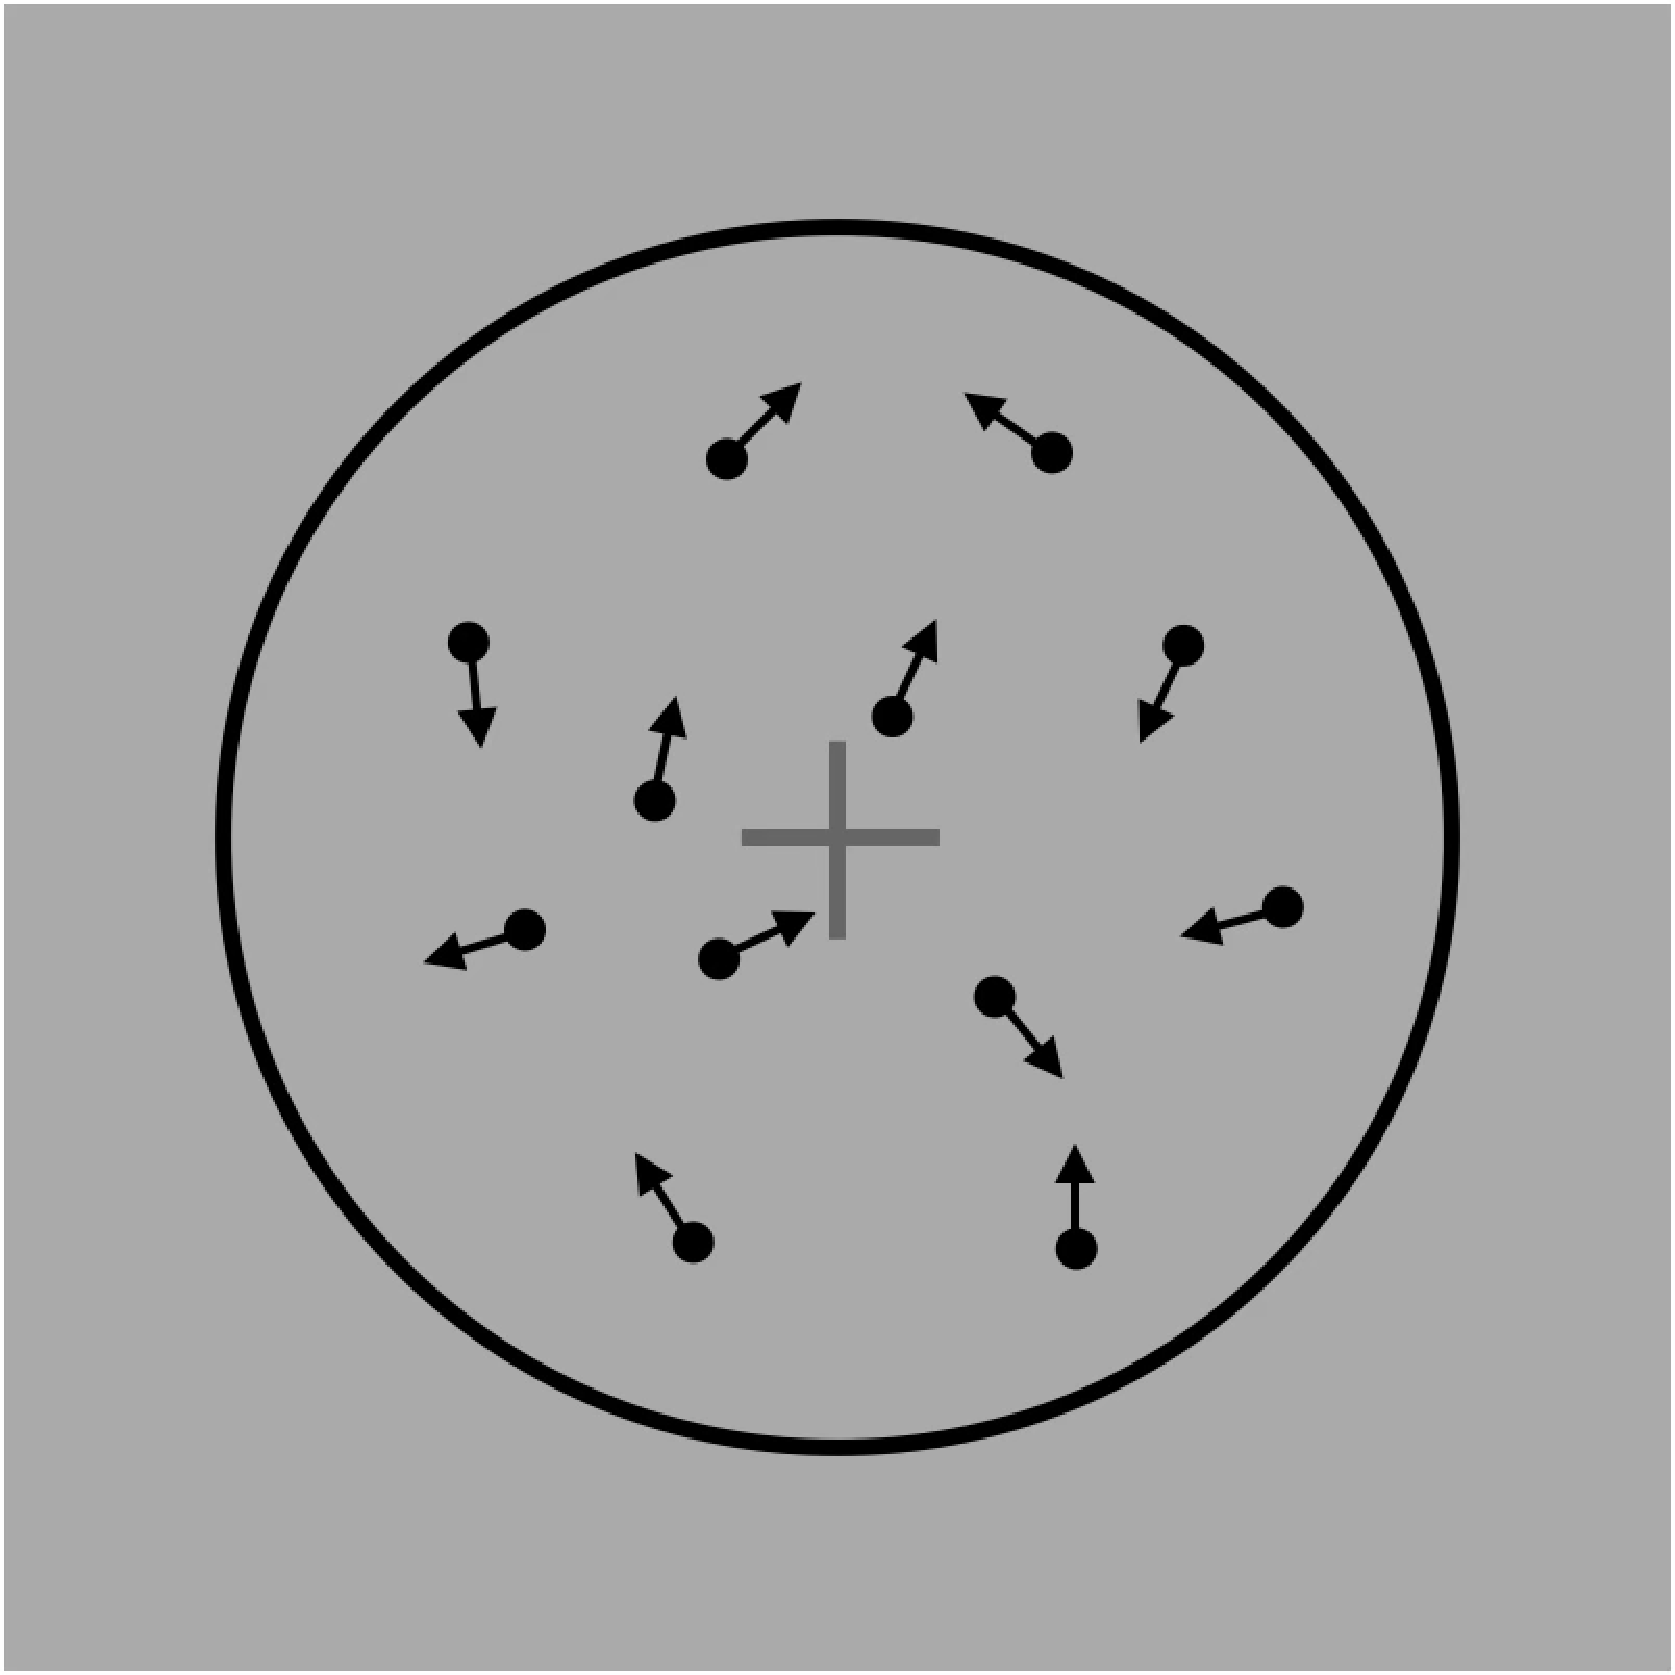
\includegraphics[width=0.2\textwidth]{../assets/rdk.pdf}
%     \caption{ランダムドットキネマトグラム刺激の例．}
%     \label{fig:rdk_stimulus}
% \end{figure}
\begin{figure*}[t]
    \centering
    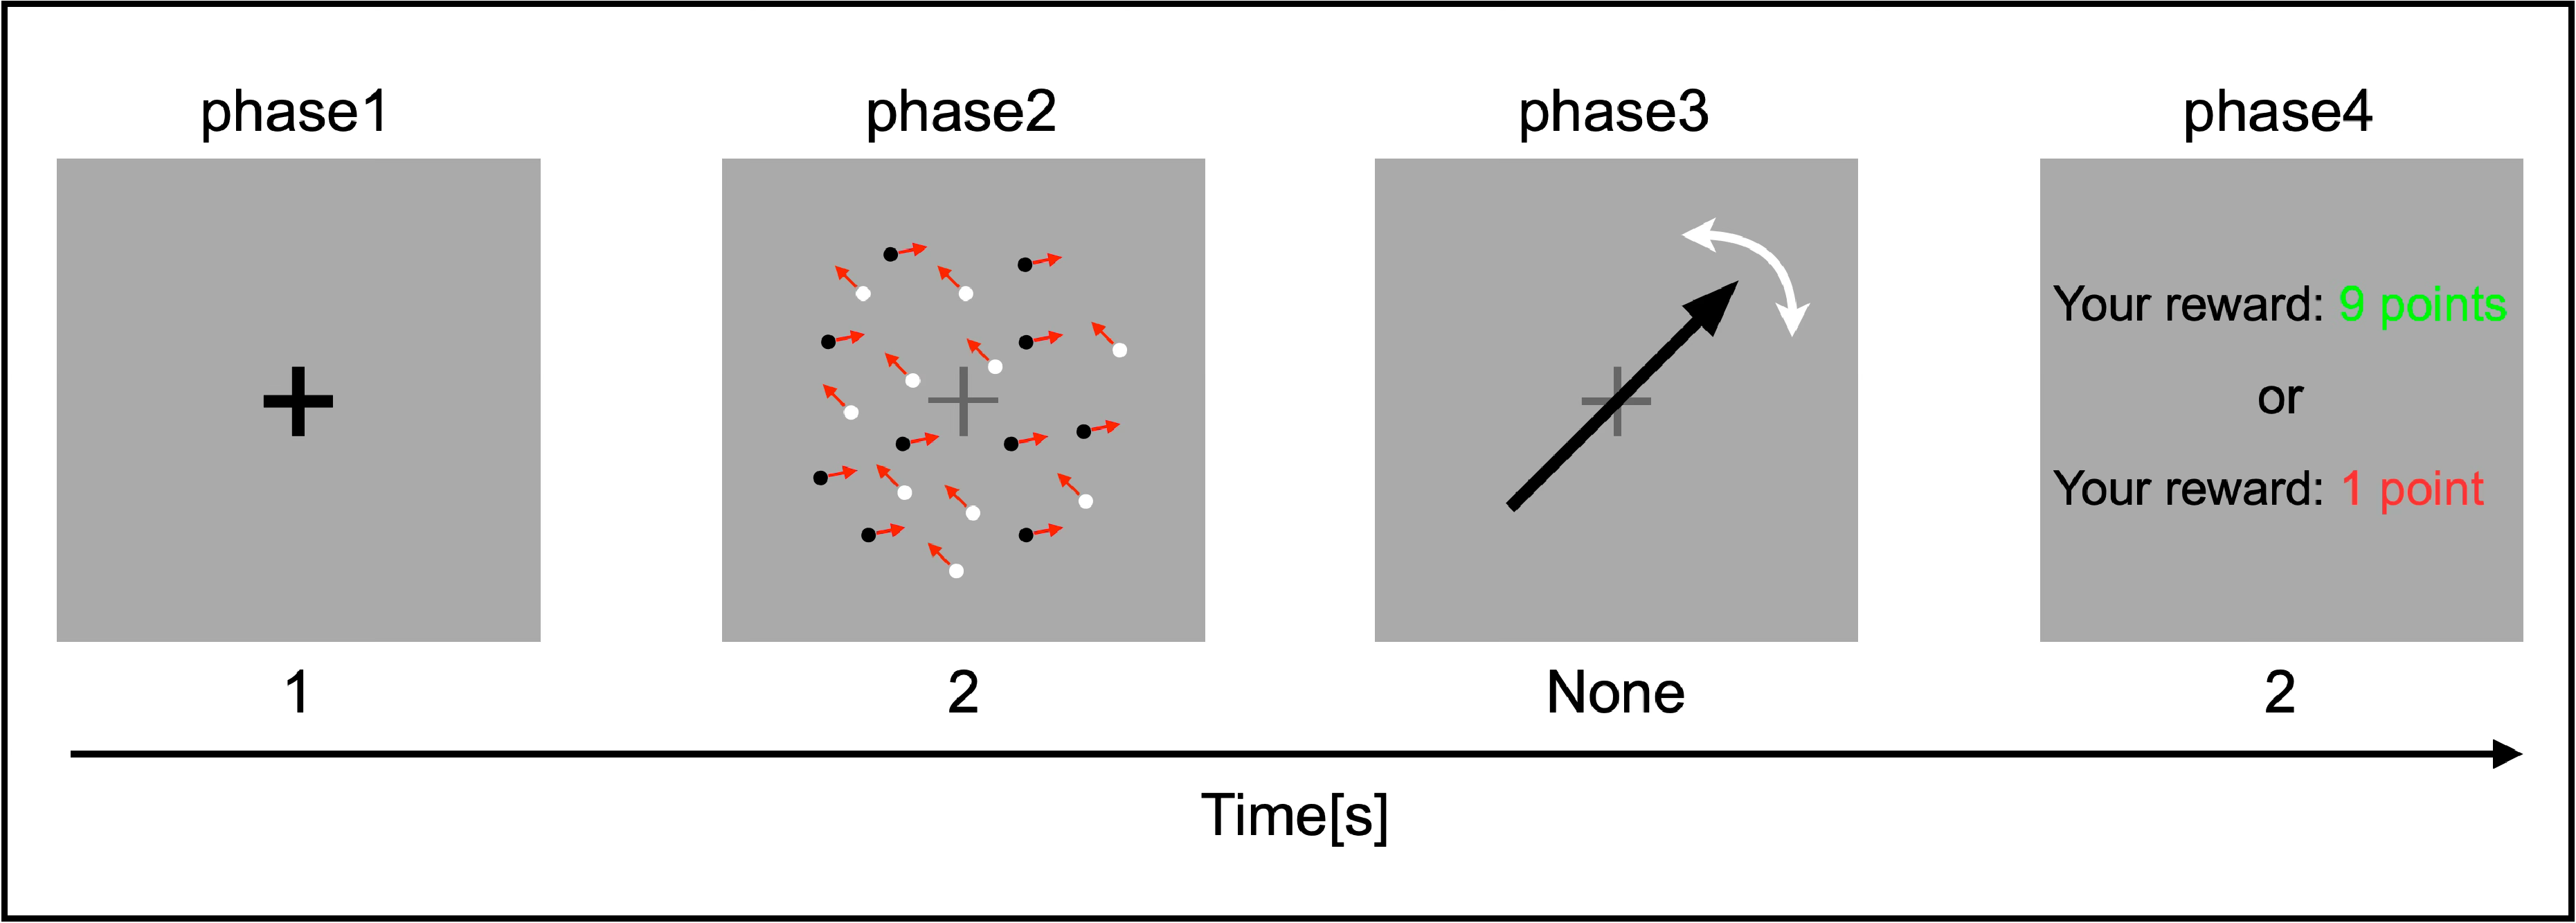
\includegraphics[width=1.0\textwidth]{../assets/dual-rdk-procedure-modified.pdf}
    \caption{実験の1回の試行の流れ．
    各フェーズの提示時間を画面下に記載している．
    フェーズ3における回答時間は無制限である．
    なお，図中の赤矢印はドット群の運動方向を示す．}
    \label{fig:experiment_procedure}
\end{figure*}
\subsection{環境}
実験は，JsPsych v2.0.0を用いて作成した．

\subsection{実験参加者}
実験参加者は合計80名で，オンライン実験ツールであるProlific~\cite{palan2018prolific}を用いて募集した．

全ての参加者は内容に同意した上で実験に参加した．本実験は，大阪大学大学院工学研究科における人を対象とした研究倫理委員会の審査を受けた（承認番号5-7-1）．

\subsection{実験手順}
実験は16試行の練習セッションと72試行の本番セッションで構成された．
実験の1回の試行を図~\ref{fig:experiment_procedure}に示す．
1試行は，固視点の提示，色（白・黒）の異なる2つのRDK刺激の同時提示，方向の回答フェーズ，そして報酬フェーズで構成された．

実験参加者には，白・黒のドット群がそれぞれ異なる方向に運動する2種類のRDK刺激を同時に提示し，
ドット数の多い方のドット群の運動方向を報告するように指示した．
つまり，この課題では，ドット数の多い刺激がターゲット刺激であり，ドット数の少ない刺激がディストラクタ刺激であった．
各試行は固視点提示（1秒），刺激提示（2秒），回答，報酬提示（2秒）の4つのフェーズで構成された．
固視点は参加者の視線を画面中央に誘導し，刺激提示前の視線のばらつきを抑制することを目的とした．
刺激提示フェーズでは白・黒のRDK刺激を同時に提示し，
回答フェーズでは，参加者には，キーボードの左右の矢印キーを用いてバーを回転させ，
その向きをドット群の運動方向に一致させるように指示した．
バーの初期位置はランダムに決定され，回答時間は無制限であった．
報酬フェーズではターゲット刺激に対する角度誤差に応じた報酬を提示した
（報酬の決定方法については\ref{sec:reward_structure}節で述べる）．
参加者には，最終的な獲得報酬に応じて実験終了後に謝金が支払われることを事前に伝えた．
実験が終了するまで約15分を要した．

\subsubsection{練習セッション}
練習セッションは16試行で構成され，バーの操作に慣れてもらうという目的のもと，
ドット数と方向はランダムに決定し，2つの輝度の異なるRDK刺激を同時表示した．
したがって，練習セッションでは，2つのドット群のドット数の差が顕著に現れる．

\subsubsection{本番セッション}
本番セッションは72試行で構成され，前半48試行はlearningステージ，後半24試行はawarenessステージとした．
% learningステージはターゲットを学習したかどうか，awarenessステージはその学習が意識的かどうかを解析することを目的とした．
本番セッションの各試行では，ドット数が同数である2つの色の異なるRDK刺激を同時表示した．
つまり，2つのRDK刺激のドット数は同数であるため，ターゲット刺激とディストラクタ刺激の区別はない．
ただし，ドット群が運動する方向は2色のドット群でそれぞれ異なり，その運動方向に応じて報酬が変化するように設定した．
したがって，本番セッションでは，参加者はドット数が多いと感じた方のドット群の運動方向を報告することを指示されたが，
実際にはドット数ではなく，運動方向によって得られる報酬が変化した．
次節では，本番セッションにおける報酬構造について述べる．

% 一方で，awarenessステージにおける刺激は，learningステージにおける刺激のターゲットとディストラクタを入れ替えたものである．
% つまり，learningステージでは図~\ref{fig:stimuli}の報酬構造を極座標の角度方向に$\pi$回転した場合の刺激が生成される．


\subsection{報酬構造}\label{sec:reward_structure}
実験の本番セッションにおける報酬構造は，参加者には明示的に伝えられておらず，
報酬をより多く獲得するためには，暗黙的に設定された報酬構造を学習する必要がある．

\begin{figure}[t]
    \centering
    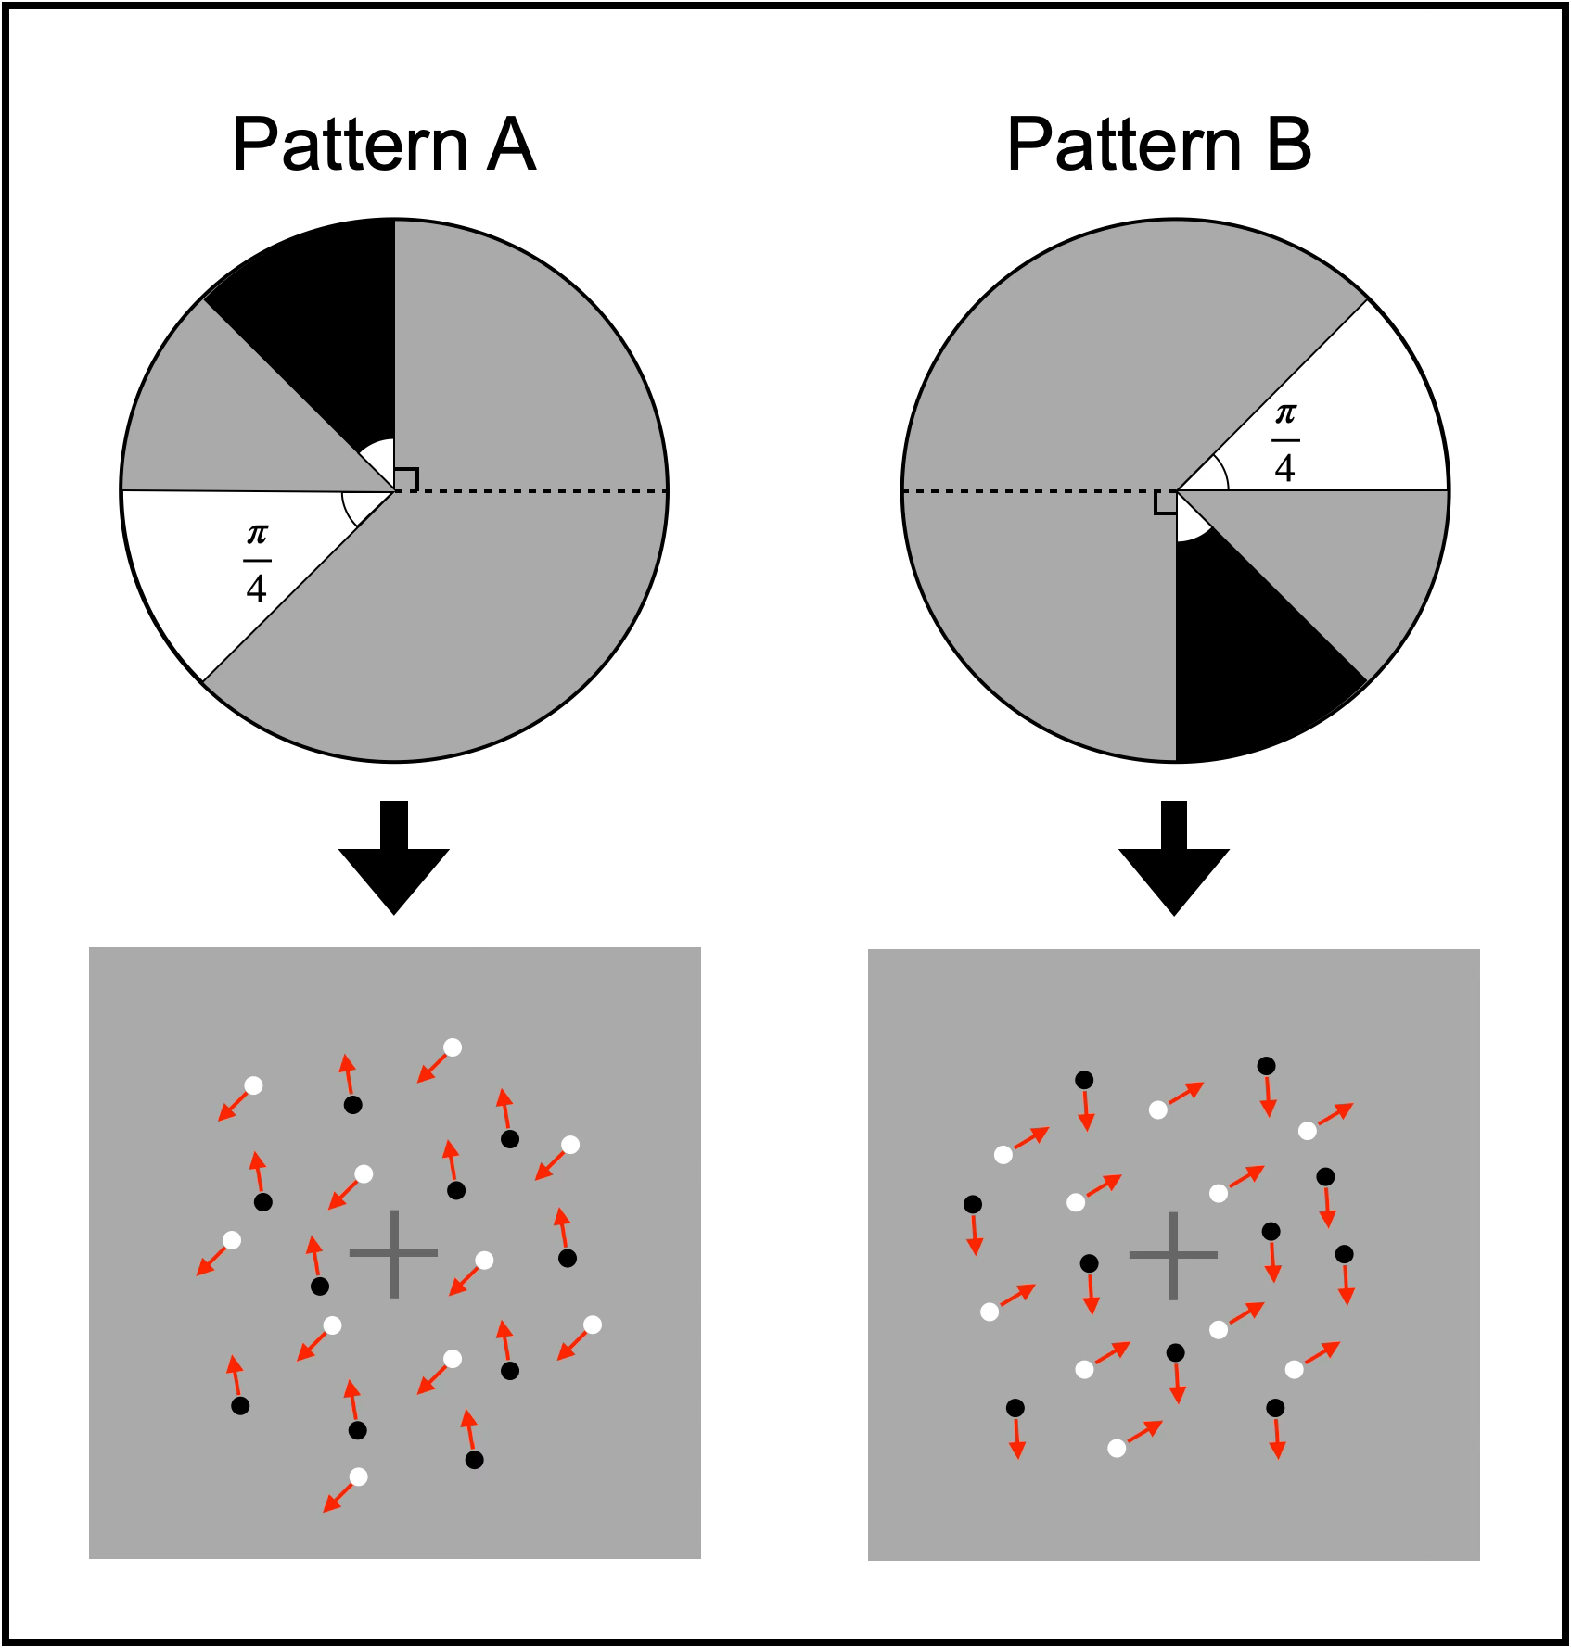
\includegraphics[width=1.0\linewidth]{../assets/learning-stimuli-modified.pdf}
    \caption{本番セッションにおける2種類の刺激パターン．
    （上段）白・黒のドット群の運動方向の発生範囲．
    （下段）刺激の具体例（赤矢印はドット群の運動方向を示す）．
    % 右側のペアの場合は白色ドット群がターゲット，黒色ドット群がディストラクタとなる\\
    % 左側は黒色ドット群がターゲット，白色ドット群がディストラクタとなる
    }
    \label{fig:stimuli}
\end{figure}
本番セッションの各試行における刺激は，高報酬刺激と低報酬刺激で構成された．
それぞれ高報酬刺激と低報酬刺激は運動方向に規則性があり，そのパターンが2種類存在した．
図~\ref{fig:stimuli}は，本番セッションにおける2種類の刺激のパターン，ドット群の運動方向の範囲，および刺激の具体例を示す．
パターンAでは，高報酬刺激は黒色ドット群であり，低報酬刺激は白色ドット群である．
逆にパターンBでは，高報酬刺激は白色ドット群であり，低報酬刺激は黒色ドット群である．
各試行では，これら2種類の刺激のパターンのうちどちらかがランダムに選択されて提示された．
それぞれの刺激の運動方向の発生範囲は$\pi/4$で，高報酬刺激と低報酬刺激の発生範囲間の角度距離は$\pi/4$である．

各試行の報酬は，回答角度がターゲットの方向角度に一致すると10点，$\pi/4$以上離れると0点になるように調整した．
これを実現するため，各試行において2つのドット群の運動方向のなす角度が常に$\pi/2$以上になるように制限を加えた．
これにより，参加者がターゲットを正確に報告した場合でも，
その回答がディストラクタの方向と混同されないことが保証される．

\subsection{ステージの設計}
本節では，本番セッションにおけるlearningステージとawarenessステージの設計について説明する．

learningステージでは，参加者が報酬構造を暗黙的に学習するかどうかを検証することを目的とした．
参加者には報酬構造の存在を明示せず，試行を重ねることで高報酬なドット群を選択する割合が増加するかどうかを学習指標として用いた．

awarenessステージでは，learningステージで生じた学習が意識的な知識に基づくものかどうかを検証することを目的とした．
そのため，awarenessステージにおける報酬構造は，
learningステージのものを極座標の角度方向に$\pi$回転させたもの，
すなわち高報酬と低報酬のドット群が入れ替わった構造とした．
learningステージで獲得した知識が意識的なものであれば，報酬構造の反転に気づき選択行動が変化すると予測される．
一方，学習が無意識的なものであれば，報酬構造の反転後も以前の選択傾向が持続すると予測される．

以降の分析では，本番セッションにおける高報酬刺激を
便宜上ターゲット刺激と呼び，
高報酬刺激を選択した割合をターゲット選択率と定義する．

\section{分析}
この章では，反応時間の前処理，角度誤差指標および学習指標の算出方法，
参加者データの除外基準，ならびに統計解析について説明する．

\subsection{反応時間の前処理}

\subsubsection{対数変換}
\begin{figure*}[t]
    \centering
    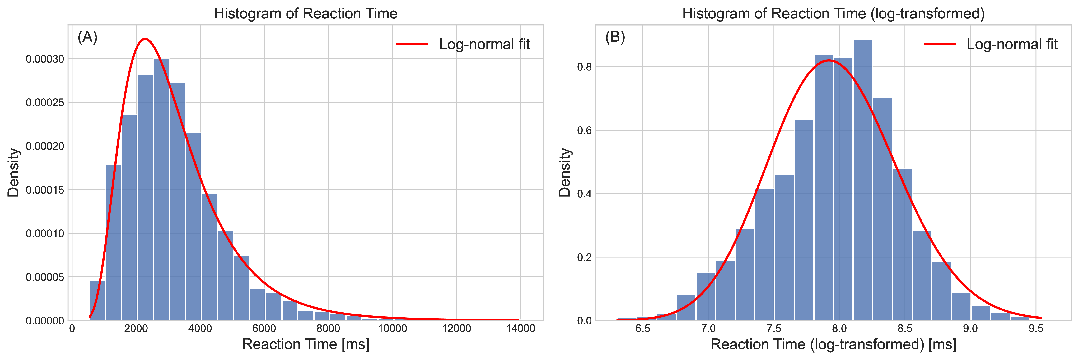
\includegraphics[width=1.0\linewidth]{../assets/rt_histogram_jointed_with_label_cropped.pdf}
    \caption{全体における反応時間のヒストグラム．}
    \label{fig:rt_distribution}
\end{figure*}
反応時間は一般に右歪みの分布を示すことが知られており，
本研究で得られた反応時間においても同様の右歪みが確認された（図~\ref{fig:rt_distribution}A）．
右歪みの分布では平均値が分布の右裾に位置する大きな値に影響されやすく，
後述する変動係数の計算における平均値の代表性を損なう可能性がある．
そのため，先行研究に倣い~\cite{gable2008approach}，
反応時間に対数変換を施し分布の対称性を高めた（図~\ref{fig:rt_distribution}B）．
以降の分析はすべて対数変換後の反応時間を用いる．

\subsubsection{変動係数の算出}
各参加者の注意状態の変動を捉える指標として，
対数変換後の反応時間の変動係数（CV）を算出した．
CVは反応時間の標準偏差を平均で割った値であり，
個人内の反応時間のばらつきを平均に対する割合で表す指標である．
式で表すと以下のようになる．
\begin{align}
    \text{CV}_\text{RT} = \frac{\sigma_{\text{RT}}}{\mu_{\text{RT}}}
\end{align}
ここで，$\sigma_{\text{RT}}$は反応時間の標準偏差，$\mu_{\text{RT}}$は反応時間の平均である．
% この指標は，反応時間のばらつきを平均に対する割合で表すものであり，個人の注意状態の変動つまり集中度を反映していると考えられる．

\subsection{角度誤差指標の算出}
知覚表現の精度を捉える指標として，角度誤差（Angle Error: AE）の絶対値の平均を算出した．
RDK課題における連続方向推定パラダイムでは，
AEは知覚精度を反映する指標として広く用いられている~\cite{bae2022perception}．
AEは，ターゲット刺激/ディストラクタ刺激の方向角度に対する回答角度の誤差を表す指標である．
各試行において，ターゲット刺激に対するAEとディストラクタ刺激に対するAEを
それぞれ算出し，値の小さい方を選択して全試行の平均を算出した．

この指標は，ターゲット刺激とディストラクタ刺激を区別なく，参加者が刺激の運動方向をどれだけ正確に報告するかを表すものである．
式で表すと以下のようになる．
\begin{align}
    \text{AE}_{\text{min}} = \frac{1}{N} \sum_{i=1}^{N} \min(|\theta_{\text{response},i} - \theta_{\text{target},i}|, |\theta_{\text{response},i} - \theta_{\text{distractor},i}|)
\end{align}
ここで，$N$は試行数，$\theta_{\text{response},i}$は$i$番目の試行における回答角度，$\theta_{\text{target},i}$はターゲット刺激の方向角度，$\theta_{\text{distractor},i}$はディストラクタ刺激の方向角度である．

\subsection{学習指標の算出}
暗黙的学習の進行を捉える指標として，
高報酬ドット群の選択率（ターゲット選択率）の変化を用いた．
ターゲット刺激の運動方向に対する回答角度の誤差が$\pi/4$未満であればターゲット選択，
ディストラクタ刺激の運動方向に対する誤差が$\pi/4$未満であればディストラクタ選択とみなした．
\ref{sec:reward_structure}節で述べた制約により2刺激の運動方向のなす角は$\pi/2$以上であるため，
両者に同時に分類される試行は存在しない．
ターゲット選択率は全試行数に対するターゲット選択試行数の割合として算出した
（どちらにも分類されない試行も分母に含む）．
学習の進行を捉えることを目的として，learningステージの前半24試行と後半24試行における
ターゲット選択率をそれぞれ算出し，その差分を学習指標とした．
差分が正の値を示す場合，課題の進行にともない高報酬ドット群を
選択する割合が増加したことを意味する．

\subsection{データの除外}
以下の4点の基準を順に適用し，該当する参加者のデータを分析から除外した．

\begin{enumerate}
\item 知覚精度に基づく除外

ターゲット刺激およびディストラクタ刺激の運動方向から
それぞれ$\pi/4$以上離れた回答の割合が30~\%以上であった参加者は，
課題に対する基本的な知覚精度が不十分であると判断し，分析から除外した．
この基準により2名を除外した．

\item 色バイアスに基づく除外

learningステージにおいて，白色または黒色のドット群のいずれかを
80~\%以上の割合で選択した参加者は，特定の色に対する強い選択バイアスを持つと判断し，
分析から除外した．
このような参加者では，ドット数や報酬構造ではなく，
色の選好が選択行動を規定している可能性がある．
この基準により15名を除外した．

\item 意識的学習に基づく除外

learningステージとawarenessステージにおいて，
試行番号を説明変数，ターゲット選択（1/0）を目的変数とした
ロジスティック回帰を行い，試行番号の回帰係数が両ステージで
有意に正であった参加者は，報酬構造を意識的に学習したと判断し，分析から除外した．
ターゲット選択（1/0）は離散的な二値データであるため，
線形回帰よりも二値の時系列データへの適合性が高いロジスティック回帰を用いた．
learningステージでは高報酬刺激への選択が試行の進行とともに増加し，
さらにawarenessステージでも反転した報酬構造に対応した選択の増加が確認される場合，
参加者が報酬構造の存在を意識的に認識し，それに基づいて選択行動を能動的に調整していたと考えられる．
本研究では暗黙的学習を検討対象としているため，
意識的な知識に基づいて選択行動を変化させた参加者は分析の対象外とした．
この基準により2名を除外した．

\item 反応時間の変動に基づく除外

上記3つの基準による除外後の参加者データをもとにCVを算出した．
CVの分布において上位10~\%の参加者は，
他の参加者と比較して著しく高い反応時間の変動を示しており，
課題に対して適切に取り組めていない可能性がある．
そのため，CVが0.9分位点を超えた参加者を分析から除外した．
この基準により7名を除外した．

\end{enumerate}

以上の基準を順に適用した結果，合計26名が除外され，
最終的な分析対象は54名となった．

\subsection{統計解析}
CVが知覚精度とは独立に学習の進行に関連するかどうかを検証するため，
CV，角度誤差指標（$\text{AE}_{\text{min}}$），学習指標（ターゲット選択率の差）の三者間の関係をそれぞれ線形回帰分析により検討した．
具体的には，CVと角度誤差指標，CVと学習指標，および角度誤差指標と学習指標の
それぞれの組み合わせについて分析を行った．
有意水準は$\alpha = 0.05$とした．

\section{結果}
\begin{figure}[t]
    \centering
    
\includegraphics[width=1.0\linewidth]{../../outputs/figures/rt_cv_vs_minimum_angular_error.pdf}
    \caption{反応時間の変動と角度誤差指標の関係．}
    \label{fig:cv_vs_minimum_ae}
\end{figure}
まず，CVと角度誤差指標（$\text{AE}_{\text{min}}$）との関係を線形回帰分析した結果，
CVは$\text{AE}_{\text{min}}$を有意に予測した（$p = 0.025$，図~\ref{fig:cv_vs_minimum_ae}）．
すなわち，反応時間の変動が大きい参加者ほど，平均的な報告角度誤差指標が大きい傾向が認められた．

\begin{figure}[t]
    \centering
    
\includegraphics[width=1.0\linewidth]{../../outputs/figures/rt_cv_vs_target_choice_rate_diff.pdf}
    \caption{CVと学習指標の関係．}
    \label{fig:cv_vs_target_choice_rate_diff}
\end{figure}
続いて，CVと学習指標（ターゲット選択率の差）との関係を線形回帰分析した結果，
CVは学習指標を有意に予測した（$p = 0.036$，図~\ref{fig:cv_vs_target_choice_rate_diff}）．
すなわち，反応時間の変動が大きい参加者ほど，課題の進行にともないターゲット刺激を選択する割合が増加する傾向が認められた．

\begin{figure}[t]
    \centering
    
\includegraphics[width=1.0\linewidth]{../../outputs/figures/minimum_angular_error_vs_target_choice_rate_diff.pdf}
    \caption{角度誤差指標と学習指標の関係．}
    \label{fig:minimum_ae_vs_target_choice_rate_diff}
\end{figure}
一方，角度誤差指標と学習指標との間には有意な線形関係は認められなかった（$p = 0.87$，図~\ref{fig:minimum_ae_vs_target_choice_rate_diff}）．

\section{議論}
本研究では，集中度（注意状態）の個人差が学習の進行に影響を及ぼすと仮定し，集中度を反映する指標である反応時間の変動と暗黙的学習の関係を検討した．
本研究の結果は，反応時間の変動が大きい参加者は，平均的な知覚精度が低い傾向にある一方で，課題の進行にともなうターゲット選択率の増加が大きいことを示した．
この結果は，反応時間の変動は単なるタスクパフォーマンスの低下を反映するだけでなく，
学習過程の初期状態や変化量とも関係する可能性を示している．

まず，反応時間の変動と知覚精度の関係は，反応時間の変動がタスク遂行の安定性，そして注意状態を反映している可能性を示唆した．
本研究では，反応時間の変動が大きい参加者ほど平均的な報告角度誤差が大きい傾向にあることが確認された．
この結果は，反応時間の試行間変動がタスク遂行の不安定性を反映することを示している．
先行研究において，持続的な注意の制御は時間的に揺らぎ，その揺らぎが大きい状態ではタスク遂行が不安定になることが示されている~\cite{west2002lapses}．
また，Leszczynskiら~\cite{leszczynski2017mind}は，反応時間の個人内変動を注意の逸脱や実行制御の変動を反映する指標として用い，
注意が逸脱状態にあるときの反応時間の分散の増加を報告している．
なお，反応時間の変動が試行ごとの難易度の個人差を反映している可能性を排除するため，
回答バーの初期角度と2つの刺激のうち近い方との角度差分の絶対値を難易度指標として定義し，
その個人内変動係数と反応時間の変動係数との関係を検討した．
両者の間に有意な関係は認められなかったことから（$p = 0.39$），
反応時間の変動は試行難易度の個人差を反映するものではないと言える．
本研究の結果はこれら先行研究の知見と整合しており，反応時間の変動が注意状態の変動を反映している可能性を支持する．

%%反応時間の変動がどのようにして注意状態を反映しているのかの解釈
% さらに，ramchurnら~\cite{ramchurn2014intraindividual}は，反応時間の個人内変動の増加は，
% 全体的な反応時間の遅延ではなく断続的に生じる遅い反応の増加により生じ，これは注意の逸脱や実行制御の変動を反映していると指摘している．
% これらの知見は，本研究における反応時間の変動が集中度（注意状態）を反映するという仮説を支持している．

次に，反応時間の変動と学習指標の関係は，反応時間の変動は学習能力そのものよりも，
学習過程の初期条件や変化量と関係している可能性を示唆した．
反応時間の変動が大きい参加者は，課題の進行にともないターゲット刺激を選択する割合が有意に増加することが確認された．
この結果は，反応時間の試行間変動が学習の進行に関連している可能性を示している．
ただし，学習指標として定義したターゲット選択率の差分は，タスク前半とタスク後半の選択率の差を表すものであり，
その増加が後半における選択率の上昇に起因するのか，前半における選択率の低さに起因するのかを区別することはできない．
この点を検討するため，反応時間の変動とタスク前半のターゲット選択率の関係を線形回帰分析により検討したところ，
両者の間に負の有意な関係が認められた（$p = 0.017$）．
この結果は，反応時間の変動が大きい参加者は，タスクの初期段階でターゲット刺激を選択する割合が低い傾向にあることを示している．
さらに，タスク後半における選択割合と反応時間の変動には有意な関係が確認されなかったことから，
学習指標の増加は後半における選択率の上昇よりも，前半における選択率の低さを反映している可能性が示唆される．
反応時間の変動は学習能力そのものよりも，学習過程の初期条件や変化量と関係している可能性がある．

しかし，反応時間の変動が大きい参加者において，
課題の進行にともないターゲット選択率が増加するという学習の進行そのものは否定されない．
この一見矛盾した結果，すなわち注意の不安定な参加者ほど暗黙的学習が進行しやすいという結果は，
注意の散漫状態が暗黙的処理を促進する可能性を示唆している．
マインドワンダリング研究は，注意が課題から離れた状態においてもある種の認知処理が
促進される可能性を示しており~\cite{simor2025mind,decker2023pay}，
本研究の結果はこの知見と整合する．
したがって，注意状態が集中と散漫の間を動的に遷移する参加者は，
散漫状態において課題に対する意識的な関与が低下する一方で，
暗黙的な報酬構造の学習が促進された可能性がある．

本研究では，集中度（注意状態）の個人差が学習の進行に影響を及ぼすという仮説を部分的に支持した．
ただし，現時点の結果は学習能力そのものよりも，学習過程の初期条件や進行の仕方に関する個人差を表している可能性がある．
反応時間の変動を注意状態の直接的な指標とみなすことには限界があるため，今後の研究では，trial-levelの変動やより直接的な注意指標を組み合わせて検討する必要がある．

\section*{謝辞}
本研究の一部はJSPS科研費26H02536，25K16015，22H05163，24K15047の助成を受けたものである．

\bibliographystyle{sieicej}
\bibliography{myrefs}
% \begin{thebibliography}{97}% 文献数が10未満の時 {9}
% \bibitem{}
% \end{thebibliography}

\end{document}
